% =====================================================================
%  CMOS VLSI Lab (ECEL23606) - Textbook Schematics, Stick Diagrams
%  and Layouts for the three analog experiments.
%
%  HOW TO USE IN OVERLEAF:
%   1. Create a new Overleaf project, paste this whole file into main.tex.
%   2. Set the compiler to pdfLaTeX (Menu -> Compiler -> pdfLaTeX).
%   3. Compile. You get one PDF with all 8 figures, each on its own block.
%   4. To use a single figure in your report, copy the tikzpicture (or the
%      whole figure environment) into your own document that loads:
%         \usepackage{circuitikz}
%         \usepackage{tikz}
%         \usetikzlibrary{calc}
%
%  COLOUR CONVENTION used in the stick diagrams & layouts (Mead-Conway style):
%     Metal1 = blue,  Polysilicon = red,  n-diffusion = green,
%     p-diffusion = orange,  Contact = black square,  n-well = dashed box,
%     Select/implant = dotted box.
% =====================================================================
\documentclass[11pt]{article}
\usepackage[a4paper,margin=2cm]{geometry}
\usepackage{circuitikz}
\usepackage{tikz}
\usetikzlibrary{calc}
\usepackage{amsmath}

% ---- shared layer styles for stick diagrams and layouts ----
\tikzset{
  metalS/.style ={blue, line width=4pt, line cap=rect, opacity=0.65},
  polyS/.style  ={red, line width=4pt, line cap=rect, opacity=0.8},
  ndiffS/.style ={green!55!black, line width=7pt, line cap=rect, opacity=0.55},
  pdiffS/.style ={orange!85!yellow, line width=7pt, line cap=rect, opacity=0.7},
  contact/.style={draw=black, fill=black, minimum size=6pt, inner sep=0pt},
  nwellS/.style ={dashed, draw=black!60, line width=0.8pt},
  nwell/.style  ={draw=blue!50, dashed, line width=1pt, fill=blue!6},
  active/.style ={draw=green!55!black, fill=green!55, fill opacity=0.45},
  poly/.style   ={draw=red!70!black,  fill=red!75,   fill opacity=0.55},
  metal/.style  ={draw=blue!70!black, fill=blue!55,  fill opacity=0.40},
  cont/.style   ={draw=black, fill=black},
  sel/.style    ={draw=#1, dotted, line width=1pt},
}

\title{CMOS VLSI Lab (ECEL23606)\\ Schematics, Stick Diagrams and Layouts}
\author{Analog experiments: Inverter, 2-input NAND, Common-Source Amplifier}
\date{}

\begin{document}
\maketitle

% =====================================================================
\section{CMOS Inverter}
% =====================================================================

\subsection*{1.1 Schematic}
\begin{figure}[h]\centering
\begin{circuitikz}[scale=1.2, transform shape]
  % --- transistors ---
  \node[pmos, yscale=-1] (P) at (0,2.1) {};   % flipped: source on top
  \node[nmos]            (N) at (0,-0.4) {};
  % --- supply rails ---
  \draw (P.S) -- (0,3.3) node[vcc]{$V_{DD}$};
  \draw (N.S) -- (0,-1.6) node[ground]{};
  % --- output column (drain to drain) ---
  \draw (P.D) -- (N.D);
  \coordinate (mid) at ($(P.D)!0.5!(N.D)$);
  \draw (mid) -- (2.2,0);
  \node[ocirc] at (2.2,0) {};  \node[right] at (2.3,0) {$V_{out}$};
  % --- input (gates tied) ---
  \draw (P.G) -- (-1.3, 2.1);
  \draw (N.G) -- (-1.3,-0.4);
  \draw (-1.3,2.1) -- (-1.3,-0.4);
  \draw (-1.3,0.85) -- (-2.4,0.85);
  \node[ocirc] at (-2.4,0.85) {}; \node[left] at (-2.5,0.85) {$V_{in}$};
  \node[right] at (P.D) {\scriptsize PMOS};
  \node[right] at (N.D) {\scriptsize NMOS};
\end{circuitikz}
\caption{CMOS inverter schematic.}
\end{figure}

\subsection*{1.2 Stick diagram}
\begin{figure}[h]\centering
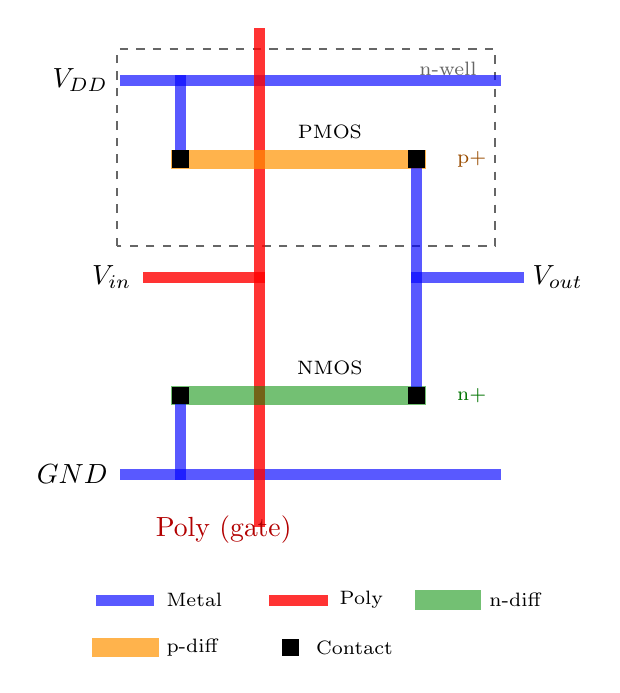
\begin{tikzpicture}[scale=1.0]
  \draw[nwellS] (0.2,2.9) rectangle (5.0,5.4);
  \node[black!60] at (4.4,5.15) {\scriptsize n-well};
  \draw[metalS] (0.3,5) -- (5,5);   \node[left] at (0.2,5) {$V_{DD}$};
  \draw[metalS] (0.3,0) -- (5,0);   \node[left] at (0.2,0) {$GND$};
  \draw[polyS] (2,-0.6) -- (2,5.6);
  \node[red!70!black] at (1.55,-0.7) {Poly (gate)};
  \draw[polyS] (2,2.5) -- (0.6,2.5);
  \node[left] at (0.5,2.5) {$V_{in}$};
  \draw[pdiffS] (1,4) -- (4,4);   \node[orange!60!black] at (4.7,4) {\scriptsize p+};
  \draw[ndiffS] (1,1) -- (4,1);   \node[green!45!black]  at (4.7,1) {\scriptsize n+};
  \draw[metalS] (1,5) -- (1,4);   \draw[metalS] (1,0) -- (1,1);
  \node[contact] at (1,4) {}; \node[contact] at (1,1) {};
  \draw[metalS] (4,4) -- (4,1);
  \node[contact] at (4,4) {}; \node[contact] at (4,1) {};
  \draw[metalS] (4,2.5) -- (5.3,2.5);
  \node[right] at (5.35,2.5) {$V_{out}$};
  \node[black] at (2.9,4.35) {\scriptsize PMOS};
  \node[black] at (2.9,1.35) {\scriptsize NMOS};
  \begin{scope}[shift={(0,-2.2)}]
    \draw[metalS]  (0,0.6)--(0.6,0.6); \node[right] at (0.7,0.6){\scriptsize Metal};
    \draw[polyS]   (2.2,0.6)--(2.8,0.6); \node[right] at (2.9,0.6){\scriptsize Poly};
    \draw[ndiffS]  (4.1,0.6)--(4.7,0.6); \node[right] at (4.8,0.6){\scriptsize n-diff};
    \draw[pdiffS]  (0,0.0)--(0.6,0.0); \node[right] at (0.7,0.0){\scriptsize p-diff};
    \node[contact] at (2.4,0.0){}; \node[right] at (2.6,0.0){\scriptsize Contact};
  \end{scope}
\end{tikzpicture}
\caption{CMOS inverter stick diagram.}
\end{figure}

\subsection*{1.3 Layout}
\begin{figure}[h]\centering
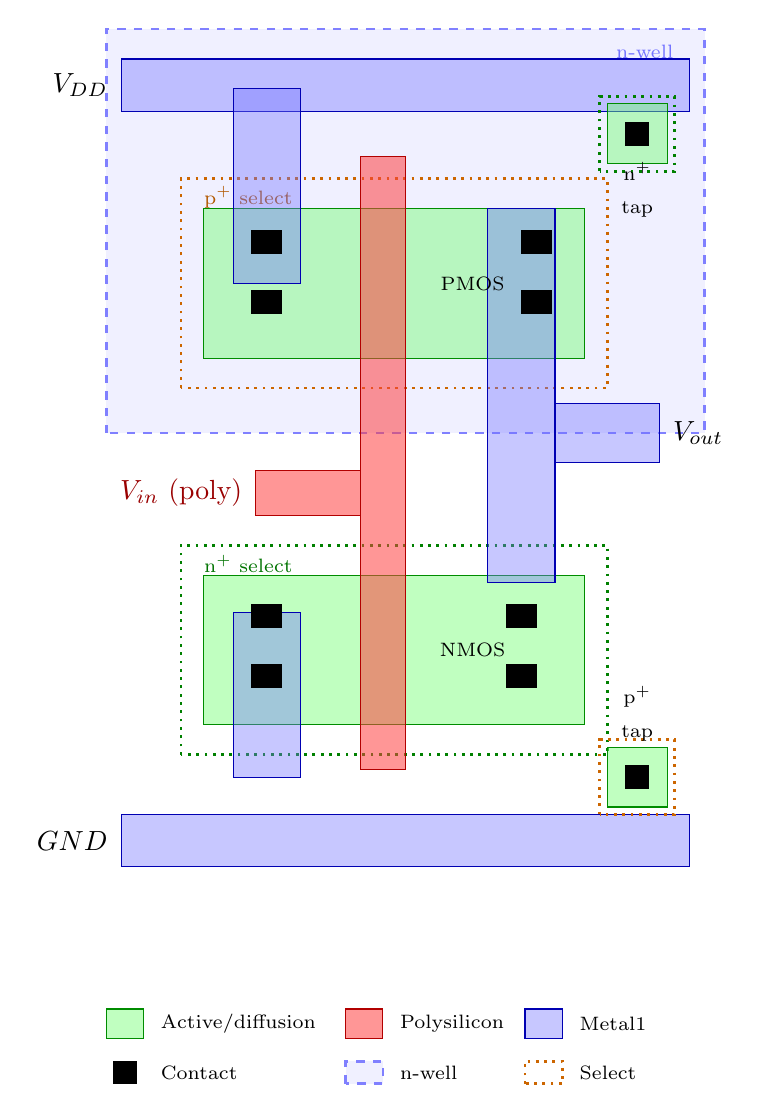
\begin{tikzpicture}[scale=0.95]
  \fill[nwell] (0.0,6.0) rectangle (8.0,11.4);
  \node[blue!55] at (7.2,11.1) {\scriptsize n-well};
  \draw[sel=orange!80!black] (1.0,6.6) rectangle (6.7,9.4);
  \node[orange!70!black] at (1.9,9.15) {\scriptsize p$^{+}$ select};
  \draw[sel=green!50!black] (1.0,1.7) rectangle (6.7,4.5);
  \node[green!45!black] at (1.9,4.25) {\scriptsize n$^{+}$ select};
  \fill[metal] (0.2,10.3) rectangle (7.8,11.0); \node[left] at (0.15,10.65){$V_{DD}$};
  \fill[metal] (0.2,0.2)  rectangle (7.8,0.9);   \node[left] at (0.15,0.55){$GND$};
  \fill[active] (1.3,7.0) rectangle (6.4,9.0);
  \fill[active] (1.3,2.1) rectangle (6.4,4.1);
  \fill[poly] (3.4,1.5) rectangle (4.0,9.7);
  \fill[poly] (3.4,4.9) rectangle (2.0,5.5);
  \node[red!60!black,left] at (1.95,5.2) {$V_{in}$ (poly)};
  \fill[metal] (1.7,8.0) rectangle (2.6,10.6);
  \fill[metal] (5.1,4.0) rectangle (6.0,9.0);
  \fill[metal] (1.7,1.4) rectangle (2.6,3.6);
  \fill[metal] (6.0,5.6) rectangle (7.4,6.4); \node[right] at (7.45,6.0){$V_{out}$};
  \foreach \y in {7.6,8.4}{ \fill[cont] (1.95,\y) rectangle (2.35,\y+0.3); }
  \foreach \y in {7.6,8.4}{ \fill[cont] (5.55,\y) rectangle (5.95,\y+0.3); }
  \foreach \y in {2.6,3.4}{ \fill[cont] (1.95,\y) rectangle (2.35,\y+0.3); }
  \foreach \y in {2.6,3.4}{ \fill[cont] (5.35,\y) rectangle (5.75,\y+0.3); }
  \fill[active] (6.7,9.6) rectangle (7.5,10.4);
  \draw[sel=green!50!black] (6.6,9.5) rectangle (7.6,10.5);
  \fill[cont] (6.95,9.85) rectangle (7.25,10.15);
  \node[align=center] at (7.1,9.25) {\scriptsize n$^{+}$\\\scriptsize tap};
  \fill[active] (6.7,1.0) rectangle (7.5,1.8);
  \draw[sel=orange!80!black] (6.6,0.9) rectangle (7.6,1.9);
  \fill[cont] (6.95,1.25) rectangle (7.25,1.55);
  \node[align=center] at (7.1,2.25) {\scriptsize p$^{+}$\\\scriptsize tap};
  \node[black] at (4.9,8.0) {\scriptsize PMOS};
  \node[black] at (4.9,3.1) {\scriptsize NMOS};
  \begin{scope}[shift={(0,-2.6)}]
    \fill[active](0,0.5) rectangle(0.5,0.9); \node[right] at(0.6,0.7){\scriptsize Active/diffusion};
    \fill[poly]  (3.2,0.5) rectangle(3.7,0.9); \node[right] at(3.8,0.7){\scriptsize Polysilicon};
    \fill[metal] (5.6,0.5) rectangle(6.1,0.9); \node[right] at(6.2,0.7){\scriptsize Metal1};
    \fill[cont]  (0.1,-0.1) rectangle(0.4,0.2); \node[right] at(0.6,0.05){\scriptsize Contact};
    \draw[nwell] (3.2,-0.1) rectangle(3.7,0.2); \node[right] at(3.8,0.05){\scriptsize n-well};
    \draw[sel=orange!80!black](5.6,-0.1)rectangle(6.1,0.2);\node[right]at(6.2,0.05){\scriptsize Select};
  \end{scope}
\end{tikzpicture}
\caption{CMOS inverter layout (PMOS in n-well on top, NMOS below; poly gate, M1 routing, well/substrate taps).}
\end{figure}

\clearpage
% =====================================================================
\section{2-input CMOS NAND gate}
% =====================================================================

\subsection*{2.1 Schematic}
\begin{figure}[h]\centering
\begin{circuitikz}[scale=1.1, transform shape]
  \node[pmos, yscale=-1] (PA) at (0,3.0) {};
  \node[pmos, yscale=-1] (PB) at (3.0,3.0) {};
  \draw (PA.S) -- (0,5.4);  \draw (PB.S) -- (3.0,5.4);
  \draw (0,5.4) -- (3.0,5.4);
  \draw (1.5,5.4) -- (1.5,5.9) node[vcc]{$V_{DD}$};
  \draw (PA.D) -- (0,2.0);  \draw (PB.D) -- (3.0,2.0);
  \draw (0,2.0) -- (3.0,2.0);
  \node[circ] at (1.5,2.0) {};
  \draw (3.0,2.0) -- (4.7,2.0); \node[ocirc] at (4.7,2.0){}; \node[right] at (4.8,2.0){$Y$};
  \node[nmos] (NA) at (1.5,0.6) {};
  \node[nmos] (NB) at (1.5,-1.7) {};
  \draw (1.5,2.0) -- (NA.D);
  \draw (NA.S) -- (NB.D);
  \draw (NB.S) -- (1.5,-3.1) node[ground]{};
  \draw (PA.G) -- (-1.6,3.0);
  \draw (NA.G) -- (-1.6,0.6);  \node[circ] at (-1.6,0.6){};
  \draw (-1.6,3.0) -- (-1.6,-0.4);
  \node[ocirc] at (-1.6,-0.4){}; \node[below] at (-1.6,-0.55){$A$};
  \draw (PB.G) -- (2.0,3.0) -- (2.0,6.2) -- (-2.6,6.2) -- (-2.6,-1.7);
  \draw (NB.G) -- (-2.6,-1.7); \node[circ] at (-2.6,-1.7){};
  \draw (-2.6,-1.7) -- (-2.6,-2.4);
  \node[ocirc] at (-2.6,-2.4){}; \node[below] at (-2.6,-2.55){$B$};
  \node[left]  at (PA.bulk) {\scriptsize $P_A$};
  \node[right] at (PB.bulk) {\scriptsize $P_B$};
  \node[right] at (NA.bulk) {\scriptsize $N_A$};
  \node[right] at (NB.bulk) {\scriptsize $N_B$};
\end{circuitikz}
\caption{2-input CMOS NAND schematic (PMOS in parallel, NMOS in series). The only
wire crossing is signal $B$ over the $V_{DD}$ rail (no connection).}
\end{figure}

\subsection*{2.2 Stick diagram}
\begin{figure}[h]\centering
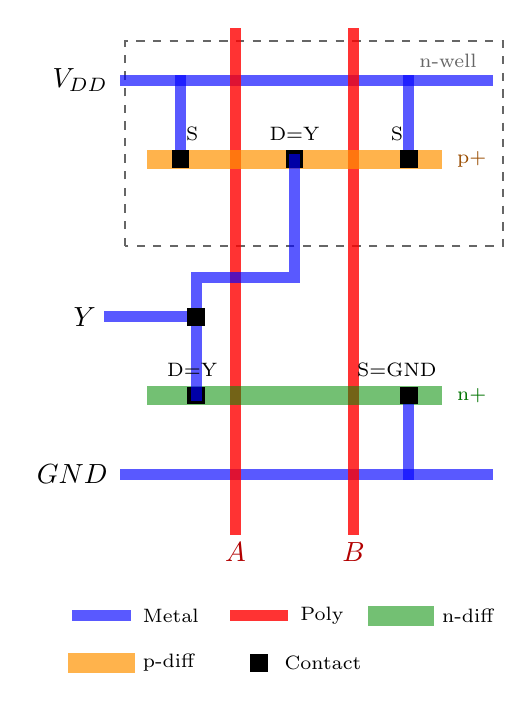
\begin{tikzpicture}[scale=1.0]
  \draw[nwellS] (0.6,2.9) rectangle (5.4,5.5);
  \node[black!60] at (4.7,5.25) {\scriptsize n-well};
  \draw[metalS] (0.6,5) -- (5.2,5);  \node[left] at (0.5,5){$V_{DD}$};
  \draw[metalS] (0.6,0) -- (5.2,0);  \node[left] at (0.5,0){$GND$};
  \draw[polyS] (2.0,-0.7) -- (2.0,5.6);  \node[red!70!black,below] at (2.0,-0.75){$A$};
  \draw[polyS] (3.5,-0.7) -- (3.5,5.6);  \node[red!70!black,below] at (3.5,-0.75){$B$};
  \draw[pdiffS] (1.0,4) -- (4.5,4);  \node[orange!60!black] at (5.0,4){\scriptsize p+};
  \draw[ndiffS] (1.0,1) -- (4.5,1);  \node[green!45!black] at (5.0,1){\scriptsize n+};
  \draw[metalS] (1.3,5)--(1.3,4);  \node[contact] at (1.3,4){};
  \draw[metalS] (4.2,5)--(4.2,4);  \node[contact] at (4.2,4){};
  \draw[metalS] (4.2,0)--(4.2,1);  \node[contact] at (4.2,1){};
  \node[contact] at (2.75,4){};
  \node[contact] at (1.5,1){};
  \draw[metalS] (2.75,4) -- (2.75,2.5) -- (1.5,2.5) -- (1.5,1);
  \draw[metalS] (1.5,2.0) -- (0.4,2.0); \node[contact] at (1.5,2.0){};
  \node[left] at (0.35,2.0) {$Y$};
  \node[black] at (1.45,4.32){\scriptsize S}; \node[black] at (2.75,4.32){\scriptsize D=Y};
  \node[black] at (4.05,4.32){\scriptsize S};
  \node[black] at (1.45,1.32){\scriptsize D=Y}; \node[black] at (4.05,1.32){\scriptsize S=GND};
  \begin{scope}[shift={(0,-2.3)}]
    \draw[metalS]  (0,0.5)--(0.6,0.5); \node[right] at (0.7,0.5){\scriptsize Metal};
    \draw[polyS]   (2.0,0.5)--(2.6,0.5); \node[right] at (2.7,0.5){\scriptsize Poly};
    \draw[ndiffS]  (3.8,0.5)--(4.4,0.5); \node[right] at (4.5,0.5){\scriptsize n-diff};
    \draw[pdiffS]  (0,-0.1)--(0.6,-0.1); \node[right] at (0.7,-0.1){\scriptsize p-diff};
    \node[contact] at (2.3,-0.1){}; \node[right] at (2.5,-0.1){\scriptsize Contact};
  \end{scope}
\end{tikzpicture}
\caption{2-input NAND stick diagram. The two PMOS share the p-diffusion (sources
to $V_{DD}$, common drain $Y$ in the middle); the two NMOS share the n-diffusion in
series (drain $Y$, internal node, source to $GND$).}
\end{figure}

\subsection*{2.3 Layout}
\begin{figure}[h]\centering
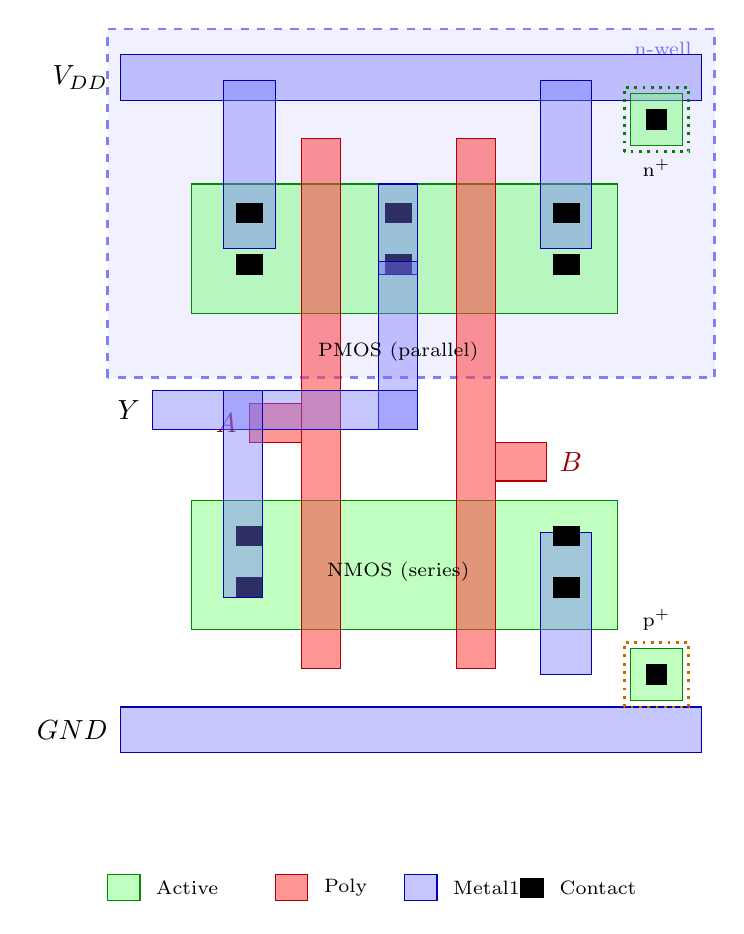
\begin{tikzpicture}[scale=0.82]
  \fill[nwell] (0.0,6.0) rectangle (9.4,11.4);
  \node[blue!55] at (8.6,11.1) {\scriptsize n-well};
  \fill[metal] (0.2,10.3) rectangle (9.2,11.0); \node[left] at (0.15,10.65){$V_{DD}$};
  \fill[metal] (0.2,0.2)  rectangle (9.2,0.9);   \node[left] at (0.15,0.55){$GND$};
  \fill[active] (1.3,7.0) rectangle (7.9,9.0);
  \fill[active] (1.3,2.1) rectangle (7.9,4.1);
  \fill[poly] (3.0,1.5) rectangle (3.6,9.7);
  \fill[poly] (5.4,1.5) rectangle (6.0,9.7);
  \fill[poly] (3.0,5.0) rectangle (2.2,5.6); \node[red!60!black,left] at (2.15,5.3){$A$};
  \fill[poly] (6.0,4.4) rectangle (6.8,5.0); \node[red!60!black,right] at (6.85,4.7){$B$};
  \fill[metal] (1.8,8.0) rectangle (2.6,10.6);
  \foreach \y in {7.6,8.4}{\fill[cont] (2.0,\y) rectangle (2.4,\y+0.3);}
  \fill[metal] (6.7,8.0) rectangle (7.5,10.6);
  \foreach \y in {7.6,8.4}{\fill[cont] (6.9,\y) rectangle (7.3,\y+0.3);}
  \foreach \y in {7.6,8.4}{\fill[cont] (4.3,\y) rectangle (4.7,\y+0.3);}
  \fill[metal] (6.7,1.4) rectangle (7.5,3.6);
  \foreach \y in {2.6,3.4}{\fill[cont] (6.9,\y) rectangle (7.3,\y+0.3);}
  \foreach \y in {2.6,3.4}{\fill[cont] (2.0,\y) rectangle (2.4,\y+0.3);}
  \fill[metal] (4.2,7.6) rectangle (4.8,9.0);
  \fill[metal] (4.2,5.2) rectangle (4.8,7.8);
  \fill[metal] (1.8,5.2) rectangle (4.8,5.8);
  \fill[metal] (1.8,2.6) rectangle (2.4,5.8);
  \fill[metal] (0.7,5.2) rectangle (1.8,5.8); \node[left] at (0.65,5.5){$Y$};
  \fill[active] (8.1,9.6) rectangle (8.9,10.4); \draw[sel=green!50!black](8.0,9.5)rectangle(9.0,10.5);
  \fill[cont] (8.35,9.85) rectangle (8.65,10.15); \node at (8.5,9.25){\scriptsize n$^{+}$};
  \fill[active] (8.1,1.0) rectangle (8.9,1.8); \draw[sel=orange!80!black](8.0,0.9)rectangle(9.0,1.9);
  \fill[cont] (8.35,1.25) rectangle (8.65,1.55); \node at (8.5,2.25){\scriptsize p$^{+}$};
  \node[black] at (4.5,6.4){\scriptsize PMOS (parallel)};
  \node[black] at (4.5,3.0){\scriptsize NMOS (series)};
  \begin{scope}[shift={(0,-2.6)}]
    \fill[active](0,0.5) rectangle(0.5,0.9); \node[right] at(0.6,0.7){\scriptsize Active};
    \fill[poly]  (2.6,0.5) rectangle(3.1,0.9); \node[right] at(3.2,0.7){\scriptsize Poly};
    \fill[metal] (4.6,0.5) rectangle(5.1,0.9); \node[right] at(5.2,0.7){\scriptsize Metal1};
    \fill[cont]  (6.4,0.55) rectangle(6.75,0.85); \node[right] at(6.85,0.7){\scriptsize Contact};
  \end{scope}
\end{tikzpicture}
\caption{2-input NAND layout: shared p-diffusion (parallel PMOS) and shared
n-diffusion (series NMOS), two poly gates $A$,$B$, output $Y$ metal, well/substrate taps.}
\end{figure}

\clearpage
% =====================================================================
\section{Common-Source Amplifier with PMOS Current-Mirror Load}
% =====================================================================

\subsection*{3.1 Schematic}
\begin{figure}[h]\centering
\begin{circuitikz}[scale=1.15, transform shape]
  \node[pmos, yscale=-1] (M3) at (1.5,4.0) {};
  \node[pmos, yscale=-1] (M2) at (4.5,4.0) {};
  \draw (M3.S) -- (1.5,5.6);  \draw (M2.S) -- (4.5,5.6);
  \draw (1.5,5.6) -- (4.5,5.6);
  \draw (3.0,5.6) -- (3.0,6.1) node[vcc]{$V_{DD}$};
  \draw (M3.G) -- (1.0,3.0);  \draw (M2.G) -- (4.0,3.0);
  \draw (1.0,3.0) -- (4.0,3.0);
  \draw (M3.D) -- (1.5,3.0);  \node[circ] at (1.5,3.0) {};
  \draw (1.5,3.0) -- (1.5,2.4);
  \draw (1.5,2.4) to[I, l_=$I_{ref}$, invert] (1.5,0.2);
  \draw (1.5,0.2) -- (1.5,-0.4) node[ground]{};
  \node[nmos] (M1) at (4.5,1.1) {};
  \draw (M1.S) -- (4.5,-0.4) node[ground]{};
  \draw (M2.D) -- (4.5,1.1|-M1.D);
  \node[circ] at (4.5,2.4) {};
  \draw (4.5,2.4) -- (6.0,2.4);
  \draw (6.0,2.4) to[C, l=$C_L$] (6.0,-0.4) node[ground]{};
  \node[ocirc] at (6.0,2.4){}; \node[above right] at (6.0,2.45){$V_{out}$};
  \draw (M1.G) -- (2.9,1.1);
  \draw (2.9,1.1) to[sV, l_=$v_{in}$] (2.9,-0.4) node[ground]{};
  \node[left]  at (M3.bulk) {\scriptsize $M_3$};
  \node[right] at (M2.bulk) {\scriptsize $M_2$};
  \node[right] at (M1.bulk) {\scriptsize $M_1$};
\end{circuitikz}
\caption{Common-source amplifier with PMOS current-mirror load. $M_1$ is the NMOS
driver; $M_3$ (diode-connected) and $M_2$ form the mirror that supplies the active load.}
\end{figure}

\subsection*{3.2 Layout (representative)}
\begin{figure}[h]\centering
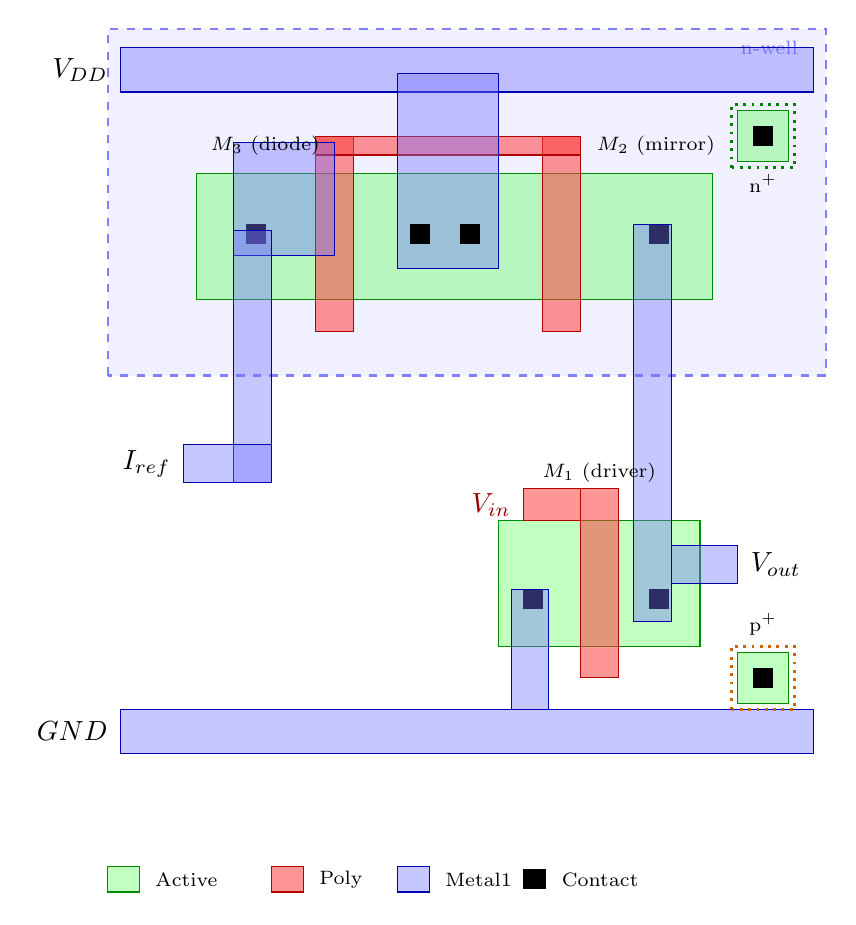
\begin{tikzpicture}[scale=0.8]
  \fill[nwell] (0.0,6.3) rectangle (11.4,11.8);
  \node[blue!55] at (10.5,11.5){\scriptsize n-well};
  \fill[metal] (0.2,10.8) rectangle (11.2,11.5); \node[left] at (0.15,11.15){$V_{DD}$};
  \fill[metal] (0.2,0.3)  rectangle (11.2,1.0);   \node[left] at (0.15,0.65){$GND$};
  \fill[active] (1.4,7.5) rectangle (9.6,9.5);
  \fill[poly] (3.3,7.0) rectangle (3.9,10.1);
  \fill[poly] (6.9,7.0) rectangle (7.5,10.1);
  \fill[poly] (3.3,9.8) rectangle (7.5,10.1);
  \fill[metal] (4.6,8.0) rectangle (6.2,11.1);
  \foreach \x in {4.8,5.6}{\fill[cont] (\x,8.4) rectangle (\x+0.3,8.7);}
  \fill[cont] (2.2,8.4) rectangle (2.5,8.7);
  \fill[metal] (2.0,8.2) rectangle (3.6,10.0);
  \fill[metal] (2.0,4.6) rectangle (2.6,8.6);
  \fill[metal] (1.2,4.6) rectangle (2.6,5.2); \node[left] at (1.15,4.9){$I_{ref}$};
  \fill[cont] (8.6,8.4) rectangle (8.9,8.7);
  \fill[active] (6.2,2.0) rectangle (9.4,4.0);
  \fill[poly]   (7.5,1.5) rectangle (8.1,4.5);
  \fill[poly]   (7.5,4.0) rectangle (6.6,4.5); \node[red!60!black,left] at (6.55,4.25){$V_{in}$};
  \fill[cont] (8.6,2.6) rectangle (8.9,2.9);
  \fill[metal] (8.35,2.4) rectangle (8.95,8.7);
  \fill[metal] (8.95,3.0) rectangle (10.0,3.6); \node[right] at (10.05,3.3){$V_{out}$};
  \fill[cont] (6.6,2.6) rectangle (6.9,2.9);
  \fill[metal] (6.4,1.0) rectangle (7.0,2.9);
  \fill[active] (10.0,9.7) rectangle (10.8,10.5); \draw[sel=green!50!black](9.9,9.6)rectangle(10.9,10.6);
  \fill[cont] (10.25,9.95) rectangle (10.55,10.25); \node at (10.4,9.35){\scriptsize n$^{+}$};
  \fill[active] (10.0,1.1) rectangle (10.8,1.9); \draw[sel=orange!80!black](9.9,1.0)rectangle(10.9,2.0);
  \fill[cont] (10.25,1.35) rectangle (10.55,1.65); \node at (10.4,2.35){\scriptsize p$^{+}$};
  \node at (2.5,9.95){\scriptsize $M_3$ (diode)};
  \node at (8.7,9.95){\scriptsize $M_2$ (mirror)};
  \node at (7.8,4.75){\scriptsize $M_1$ (driver)};
  \begin{scope}[shift={(0,-2.4)}]
    \fill[active](0,0.5) rectangle(0.5,0.9); \node[right] at(0.6,0.7){\scriptsize Active};
    \fill[poly]  (2.6,0.5) rectangle(3.1,0.9); \node[right] at(3.2,0.7){\scriptsize Poly};
    \fill[metal] (4.6,0.5) rectangle(5.1,0.9); \node[right] at(5.2,0.7){\scriptsize Metal1};
    \fill[cont]  (6.6,0.55) rectangle(6.95,0.85); \node[right] at(7.05,0.7){\scriptsize Contact};
  \end{scope}
\end{tikzpicture}
\caption{Representative transistor-level layout of the CS amplifier: PMOS mirror
$M_2$/$M_3$ share a common $V_{DD}$ source in the n-well; NMOS driver $M_1$ below;
$M_3$ is diode-connected; the two drains join at $V_{out}$.}
\end{figure}

\paragraph{Note on a ``stick diagram'' for the amplifier.}
Stick diagrams are a convention for \emph{digital} CMOS gates (inverter, NAND, NOR),
where each gate maps to a row of n-/p-diffusion crossed by poly. An analog amplifier
such as this one is not normally drawn as a stick diagram; the schematic plus the
transistor-level layout above are the standard report figures. If your examiner
insists on one, the layout above already shows the diffusion (green/orange), poly
(red) and metal (blue) ``sticks'' and can be referred to as such.

\end{document}
